\documentclass[10pt]{article}
\usepackage[a4paper,margin=18mm,top=16mm,bottom=16mm]{geometry}
\usepackage[scaled=0.92]{helvet}\renewcommand{\familydefault}{\sfdefault}
\usepackage[T1]{fontenc}\usepackage{courier}\usepackage{amsmath,booktabs,graphicx,array,xcolor,titlesec,enumitem,caption}
\titleformat{\section}{\normalsize\bfseries}{\thesection}{0.6em}{}\titlespacing*{\section}{0pt}{9pt}{3pt}
\setlength{\parindent}{0pt}\setlength{\parskip}{3pt}\captionsetup{font=small,labelfont=bf,skip=3pt}
\setlist{nosep,leftmargin=1.2em}\pagestyle{empty}
\newcommand{\pct}{\%}
\begin{document}
{\large\bfseries Size control: vertex-cap baseline against BudgetMesh}\\[1pt]
{\small 21 scenes, one target per dataset: 10~MB (13 captured scenes), 2.5~MB (8 objects). Same codec, same fine-tuning, one L40S GPU. All numbers are measured runs. 13 Nov 2026.}

\section{Result}
\begin{table}[h!]\centering\small
\begin{tabular}{@{}lcc@{}}
\toprule
 & Vertex cap & BudgetMesh \\
\midrule
Scenes within $\pm10\pct$ after 1 training & 15 / 21 & 20 / 21 \\
Scenes within $\pm10\pct$ after 2 trainings & 17 / 21 & -- \\
Scenes within $\pm10\pct$ after 3 trainings & 18 / 21 & -- \\
Scenes never within $\pm10\pct$ & 3 & 1 \\
Scenes within $\pm2\pct$ after 1 training & 3 / 21 & 19 / 21 \\
Size error, range over scenes (1 training) & $-39.6$ \ldots $+16.3\pct$ & $-22.6$ \ldots $+0.7\pct$ \\
Slowest scene that reached $\pm10\pct$: GPU minutes & 81 & 61 \\
Slowest scene that reached $\pm10\pct$: trainings & 2 & 1 \\
\bottomrule
\end{tabular}
\end{table}
\vspace{-6pt}
Time is training + fine-tuning + encoding. Slowest scenes: bonsai (cap), counter (BudgetMesh). BudgetMesh never retrains.

\section{Every scene that needed a retry, training by training}
\begin{table}[h!]\centering\small
\begin{tabular}{@{}llrrrrc@{}}
\toprule
scene (target) & training & cap & vertices kept & file (MB) & error & BudgetMesh \\
\midrule
\multicolumn{7}{@{}l}{\emph{never within $\pm10\pct$}}\\
drjohnson (10) & 1 & 1,081,000 & 881,894 & 11.57 & $+15.7\pct$ & 10.05 MB, $+0.5\pct$ \\
 & 2 & 902,000 & 900,413 & 11.69 & $+16.9\pct$ & \\
mic (2.5) & 1 & 174,000 & 106,744 & 2.04 & $-18.4\pct$ & 2.49 MB, $-0.4\pct$ \\
 & 2 & 247,000 & 107,011 & 2.05 & $-18.0\pct$ & \\
ficus (2.5) & 1 & 171,000 & 68,358 & 1.51 & $-39.6\pct$ & 1.93 MB, $-22.6\pct$ \\
 & 2 & 515,000 & 68,896 & 1.50 & $-40.0\pct$ & \\
\midrule
\multicolumn{7}{@{}l}{\emph{reached $\pm10\pct$ after a retry}}\\
kitchen (10) & 1 & 1,086,000 & 956,939 & 11.63 & $+16.3\pct$ & 10.07 MB, $+0.7\pct$ \\
 & 2 & 900,000 & 716,750 & 9.02 & $-9.8\pct$ & \\
bonsai (10) & 1 & 1,073,000 & 754,307 & 8.32 & $-16.9\pct$ & 9.99 MB, $-0.1\pct$ \\
 & 2 & 1,367,000 & 934,609 & 9.86 & $-1.4\pct$ & \\
lego (2.5) & 1 & 183,000 & 156,040 & 2.79 & $+11.6\pct$ & 2.49 MB, $-0.4\pct$ \\
 & 2 & 154,000 & 156,438 & 2.79 & $+11.7\pct$ & \\
 & 3 & 130,000 & 133,085 & 2.50 & $+0.2\pct$ & \\
\bottomrule
\end{tabular}
\end{table}
\vspace{-6pt}
drjohnson: a 17\pct{} smaller cap kept more vertices. mic, ficus: the cap does not bind; raising it changes nothing. lego: a 16\pct{} smaller cap gave the same mesh. Ficus cannot fill 2.5~MB with any method.

\section{How the baseline is set}
\textbf{Method.} MeshSplatting trained with its own \texttt{--max\_points} option (the vertex cap), then the same fine-tuning and the same codec as BudgetMesh.

\textbf{Prior (how the cap is chosen).} File size is fitted as a line in the cap, $\text{MB} = a\cdot\text{cap} + c$, by least squares on cap runs of \emph{other} scenes of the same kind; the test scene is left out. Then $\text{cap} = (T - c)/a$, rounded to 1,000.
\begin{itemize}
\item Captured scene: the 60 cap runs of the other 10 Mip-NeRF\,360 / T\&T scenes (6 caps each, 0.2--3.1 M). Deep Blending: all 66 runs of the 11 scenes. $a = 7.2$--$7.4$ MB per million, $c = 2.1$--$2.2$ MB. Caps chosen: 1,069,000--1,105,000.
\item Object: the 49 cap runs of the other 7 objects. $a = 8.5$--$9.1$ MB per million, $c = 0.9$--$1.0$ MB. Caps chosen: 171,000--183,000.
\end{itemize}
\textbf{Retry (fixed before the runs).} If the file misses the target by more than 10\pct: $\text{cap}_2 = \text{cap}_1\,(T - c)/(\text{MB}_1 - c)$, train again from scratch.

\begin{table}[h!]\centering\small
\begin{tabular}{@{}l>{\raggedright\arraybackslash}p{6.0cm}c>{\raggedright\arraybackslash}p{7.4cm}@{}}
\toprule
 & baseline & scenes & result (size error) \\
\midrule
A & cap, same-kind prior, 1 training & 21 & 15 within $\pm10\pct$; $-39.6$ \ldots $+16.3\pct$ \\
B & A + retry on a miss & 6 retried & 17 within $\pm10\pct$ \\
C & B + third training & lego & 18 within $\pm10\pct$ \\
D & cap, prior from the other kind (captured $\rightarrow$ lego) & 1 & $-41.8\pct$; retrained: $-21.4\pct$ \\
E & cap rescaled by target / measured size, retrained after a hit & 3 & garden $+3.0\rightarrow+16.4\pct$, truck $-0.5\rightarrow0.0\pct$, playroom $+9.6\rightarrow+16.3\pct$ \\
F & our size measurement and growth plan, MeshSplatting's triangle choice, no collapse & 4 & $-1.7$, $-7.2$, $+12.0$, $+9.6\pct$ \\
G & BudgetMesh, previous controller & 21 & 18 within $\pm10\pct$; $-21.6$ \ldots $+13.5\pct$ \\
H & BudgetMesh, final design & 21 & 20 within $\pm10\pct$; $-22.6$ \ldots $+0.7\pct$ \\
\bottomrule
\end{tabular}
\end{table}

\newpage
\section{Sensitivity of the cap}
166 cap runs in total (96 on captured scenes, 70 on objects). Same code, options and random seed in every run; only the cap differs.

\begin{table}[h!]\centering\small
\begin{tabular}{@{}lccc@{}}
\toprule
pairs of caps on the same scene, differing by at most & 1\pct & 5\pct & 25\pct \\
\midrule
pairs & 11 & 29 & 123 \\
larger cap gave a smaller or equal file & 4 & 12 & 35 \\
file changed by more than 10\pct & 2 & 8 & 42 \\
file change, range & $-23.7$ \ldots $+6.8\pct$ & $-23.7$ \ldots $+14.6\pct$ & $-23.7$ \ldots $+41.5\pct$ \\
\bottomrule
\end{tabular}
\end{table}
\vspace{-4pt}
\begin{table}[h!]\centering\small
\begin{tabular}{@{}lrrrrr@{}}
\toprule
garden, cap & 1,073,000 & 1,074,000 & 1,104,000 & 1,105,000 & 1,106,000 \\
\midrule
file (MB) & 11.64 & 11.61 & 13.30 & 10.30 & 10.15 \\
vertices kept / cap & 0.94 & 0.93 & 1.06 & 0.80 & 0.79 \\
\midrule
playroom, cap & 986,000 & 1,080,000 & 1,081,000 & 1,082,000 & 1,201,000 \\
\midrule
file (MB) & 11.64 & 10.37 & 10.96 & 11.07 & 14.60 \\
vertices kept / cap & 0.95 & 0.77 & 0.78 & 0.78 & 0.96 \\
\midrule
BudgetMesh on garden, target 10 MB, seeds 0 / 1 / 2 & \multicolumn{5}{r}{10.21 \quad 10.16 \quad 10.16 MB} \\
\bottomrule
\end{tabular}
\end{table}
\vspace{-4pt}
\begin{itemize}
\item \textbf{Size of the effect.} garden: cap $1{,}104{,}000 \rightarrow 1{,}105{,}000$ ($+0.09\pct$) moves the file $13.30 \rightarrow 10.30$~MB ($-23\pct$).
\item \textbf{Direction.} In 12 of 29 pairs of caps within 5\pct{} of each other, the larger cap gave the smaller (or the same) file.
\item \textbf{Range.} Vertices kept after training: 0.68--1.06 of the cap on captured scenes, 0.13--1.05 on objects.
\item \textbf{Why.} The cap bounds growth; stitching, opacity pruning and final cleaning act afterwards and remove a share the cap does not control. When growth stops below the cap (mic, ficus), the cap has no effect at all.
\end{itemize}

\begin{figure}[h!]\centering
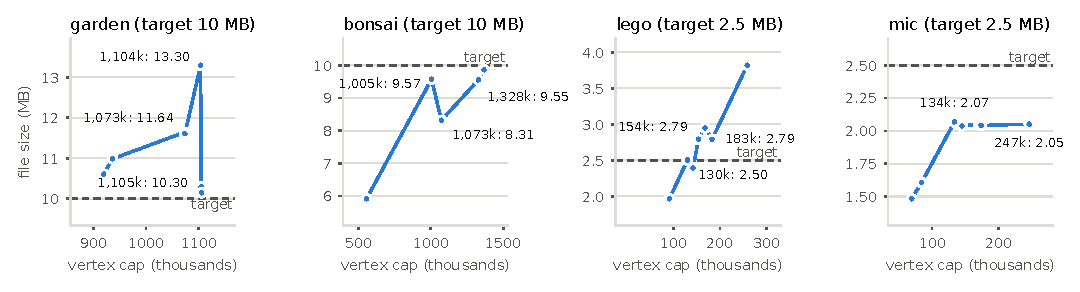
\includegraphics[width=\textwidth]{fig_cap_sensitivity.pdf}
\caption{File size against the vertex cap, all cap runs of four scenes in the shown range. Labels: cap, file size in MB.}
\end{figure}

\textbf{Limits of this report.} One target per dataset. The dense caps on garden and playroom were placed next to caps that had already behaved oddly, so the pair counts show that such jumps exist, not how often a random cap hits one. Cap runs use one seed; six cap trainings from earlier batches have no stage time stamps and are timed with the class mean (34 min captured, 18 min objects).
\end{document}
